% %! TEX root = ./main.tex
\documentclass[
   fontsize = 11pt,
   twoside = true,
   paper=a4,
   open=right
]{scrreprt}
\usepackage[utf8]{inputenc}
\usepackage[T1]{fontenc}
\usepackage{lmodern}
\usepackage{geometry}

\usepackage{tabularx}

\usepackage[ngerman]{babel}
\usepackage{csquotes}
\usepackage[
  backend=biber,
  style=numeric
]{biblatex}
\usepackage{siunitx}
\usepackage{textcomp} % für \degree

\renewcommand*{\bibfont}{\normalfont}
\addbibresource{Datasheet-Quellen/Buecher/buecher.bib}
\addbibresource{Datasheet-Quellen/Datenblaetter/datenblaetter.bib}
\addbibresource{Datasheet-Quellen/Source-Code/sourcecode.bib}
\addbibresource{Datasheet-Quellen/Webseiten/webseiten.bib}
\addbibresource{Datasheet-Quellen/Bilder/bilder.bib}

\usepackage{graphicx}
\geometry{
   %papersize={210mm, 297mm},
   includeheadfoot,
   top = 20mm,
   inner=30mm,  % größerer Bundsteg innen
   outer=20mm,  % kleinerer Rand außen
   headsep = \baselineskip,
   footskip = \dimexpr2\baselineskip+3mm\relax,
}
\usepackage{scrlayer-scrpage}
\usepackage{caption}

\captionsetup{
  justification=raggedright,
  singlelinecheck=false
}
 
\clearpairofpagestyles
 
\setkomafont{pageheadfoot}{\sffamily\footnotesize}
\setkomafont{pagehead}{\bfseries}
\setkomafont{pagination}{}

\renewcommand{\familydefault}{\sfdefault}


\KOMAoptions{
   headsepline = true,
   footsepline = true,
   plainfootsepline = true,
}


\automark[chapter]{chapter}
\ihead{\headmark}
%\ohead{\authormark}
\ofoot*{Seite~\pagemark}
\ifoot{\authormark}

\newpairofpagestyles{zusammenfassung_header_de}{
    \KOMAoptions{headsepline=false,footsepline=false,plainfootsepline=false}
   \fbox{
      \begin{minipage}[c]{0.2\textwidth}   % LINKER BLOCK
         \centering
       
\includegraphics[height=12mm]{logos/header_logo.png}
      \end{minipage}
      \begin{minipage}[c]{0.8\textwidth}   % RECHTER BLOCK
        \centering
        \textbf{HÖHERE TECHNISCHE BUNDESLEHR- UND VERSUCHSANSTALT ST. PÖLTEN}\\
        \rule{\textwidth}{0.4pt}\\[2mm]
        \textbf{Elektronik und Technische Informatik}\\
        \textbf{Ausbildungsschwerpunkt: Embedded Systems}
      \end{minipage}
      }
}
\newpairofpagestyles{zusammenfassung_header_en}{
    \KOMAoptions{headsepline=false,footsepline=false,plainfootsepline=false}
   \fbox{
      \begin{minipage}[c]{0.2\textwidth}   % LINKER BLOCK
         \centering
       
\includegraphics[height=12mm]{logos/header_logo.png}
      \end{minipage}
      \begin{minipage}[c]{0.8\textwidth}   % RECHTER BLOCK
        \centering
        \textbf{TECHNICAL AND VOCATIONAL COLLEGE ST. PÖLTEN}\\
        \rule{\textwidth}{0.4pt}\\[2mm]
        \textbf{Department: Electronics and Technical Informatics}\\
        \textbf{Educational focus: Embedded Systems / Wireless Systems}
      \end{minipage}
      }
}


\makeatletter
\newcommand*{\authormark}{}
\newcommand*{\markauthor}[1]{%
   \renewcommand{\authormark}{#1}%
   \ignorespaces
}
\newcommand*{\chapterauthor}[1]{%
   \par\vspace{-\baselineskip}%
   \textsf{von~#1}%
   \markauthor{#1}%
   \par\vspace{2\baselineskip}%
   \@afterheading
}
\makeatother
\usepackage{lipsum}

\usepackage[ngerman]{babel}  % Inhalt statt contents
\addto\captionsngerman{\renewcommand{\contentsname}{Inhalt}}

\renewcommand{\arraystretch}{1.5}

\begin{document}
\pagenumbering{arabic} % arabische Zahlen, Seitenzahl startet neu
\setcounter{page}{1}

%neues Dokument Aufbau:
%\chapter{}
%\subsection{}
% ...
%Am ende des Dokuments \newpage


\begin{titlepage}
    \thispagestyle{empty}

\noindent
\begin{minipage}[t][35mm][c]{0.18\textwidth}
    \centering
    
\includegraphics[width=\textwidth]{logos/HTL-logo.png}
\end{minipage}
\hfill
\begin{minipage}[t][35mm][c]{0.5\textwidth}
    \centering
    \textbf{\LARGE HTBLuVA St. Pölten}\\
    \textbf{Höhere Lehranstalt für}\\
    \textbf{Elektronik und Technische Informatik}\\
    Ausbildungsschwerpunkt Embedded Systems\\
    Ausbildungsschwerpunkt Wireless Systems
\end{minipage}
\hfill
\begin{minipage}[t][35mm][c]{0.18\textwidth}
    \centering
    
\includegraphics[width=\textwidth]{logos/header_logo.png}
\end{minipage}
\vspace{0.5cm}
\rule{\textwidth}{0.4pt}\\[2mm]
\vspace*{2cm}

\begin{center}
\textbf{\huge DIPLOMARBEIT}\\[1cm]

Gesamtprojekt\\[0.3cm]
\textbf{\LARGE *Titel der Diplomarbeit*}\\[0.1cm]
\end{center}
\vspace{4.3cm}
\begin{tabular}{l l l}
Ausgeführt im Schuljahr 2025/26 von: & & Betreuer:in\\
Thomas Gruber &5AHELS	 &Dipl.-Ing. Dr. XYZ\\
Matthias Greil &5BHELS &	DI (FH) RRR\\
St. Pölten, am 27. März 2026& &\\
\hline
Abgabevermerk: & & \\
\end{tabular}
\vspace{2cm}\\
\makebox[3cm]{\hrulefill} \makebox[5cm]{}\makebox[5cm]{\hrulefill}\\
\makebox[3cm][c]{\small Datum}\makebox[5cm]{} \makebox[5cm][c]{\small Betreuer:in}\\
\end{titlepage}

% Leere linke Seite erzwingen ohne Kopf-/Fußzeile und Seitenzahl
\cleardoublepage
\thispagestyle{empty}

% \cleardoublepage
% \thispagestyle{empty}
\chapter*{Eidesstattliche Erklärung:}
\thispagestyle{empty}
Ich versichere an Eides statt, dass ich diese Diplomarbeit selbstständig verfasst und keine anderen als die angegebenen Quellen und Hilfsmittel verwendet habe. Alle Gedanken, die im Wortlaut oder übernommen, oder mit künstlicher Intelligenz generiert wurde, wind ordnungsgemäß gekennzeichnet, zitiert und mit genauer Quellenangabe versehen. Die Kennzeichnung der KI-Nutzung erfolgt durch eine zusammenfassende Darstellung der verwendeten KI-Werkzeuge, der betroffenen Arbeitsbereiche. Alle übernommenen KI-generierten Inhalte und Arbeitsergebnisse habe ich eigenständig geprüft. Für ihre fachliche Richtigkeit trage ich die Verantwortung.


\vspace{5cm}
\begin{flushright}
\underline{\hspace{5cm}}\\
\makebox[5cm][c]{\small Thomas Gruber}
\\
\vspace{2cm}
\makebox[5cm]{\hrulefill}\\
\makebox[5cm][c]{\small Matthias Greil}
\end{flushright}
\newpage

%---------------------------DEUTSCH---------------------------
\thispagestyle{zusammenfassung_header_de}
\begin{center}
\vspace*{0.1cm}
\textbf{\LARGE DIPLOMARBEIT}\\
\vspace*{0.1cm}
DOKUMENTATION
\end{center}
\vspace{10pt}

\noindent\begin{tabular}{| p{0.22\textwidth} | p{0.72\textwidth}|}
    \hline
    Namen der Verfasser/innen & Name / Name \\
    \hline
    Jahrgang / Klasse / Schuljahr & 5BHELS, 2025/26\\
    \hline
    Thema der Diplomarbeit & Titel der Diplomarbeit\\
    \hline
    Kooperationspartner & Firma GMBH\\
    \hline
\end{tabular}
\par\vspace*{0.2cm}
\noindent\begin{tabular}{| p{0.22\textwidth} | p{0.72\textwidth}|}
    \hline
    Aufgabenstellung & \lipsum[1] \\
    \hline
\end{tabular}
\par\vspace*{0.2cm}
\noindent\begin{tabular}{| p{0.22\textwidth} | p{0.72\textwidth}|}
    \hline
    Realisierung & \lipsum[1] \\
    \hline
\end{tabular}
\newpage %2. Seite DEUTSCH
\thispagestyle{zusammenfassung_header_de}
\noindent\begin{tabular}{| p{0.22\textwidth} | p{0.72\textwidth}|}
    \hline
    Ergebnisse & \lipsum[1] \\
    \hline
\end{tabular}
\par\vspace*{0.2cm}
\noindent\begin{tabular}{| p{0.22\textwidth} | p{0.72\textwidth}|}
    \hline
    Grafik mit Beschreibung & \lipsum[1] \\
    \hline
\end{tabular}
\par\vspace*{0.2cm}
\noindent\begin{tabular}{| p{0.22\textwidth} | p{0.72\textwidth}|}
    \hline
    Teilnahme an Wettbewerben, Auszeichnungen & - \\
    \hline
\end{tabular}
\par\vspace*{0.2cm}
\noindent\begin{tabular}{| p{0.22\textwidth} | p{0.72\textwidth}|}
    \hline
    Möglichkeiten der Einsichtnahme in die Arbeit & - \\
    \hline
\end{tabular}
\par\vspace*{0.2cm}
\noindent\begin{tabular}{| p{0.22\textwidth} | p{0.72\textwidth}|}
    \hline
    Approbation & \\
    \footnotesize (Datum/Unterschrift) & \\
    \hline
\end{tabular}
\par\vspace*{0.2cm}
\newpage
%---------------------------Englisch---------------------------
\thispagestyle{zusammenfassung_header_en}
\begin{center}
\vspace*{0.1cm}
\textbf{\LARGE DIMPLOMA THESIS}\\
\vspace*{0.1cm}
DOCUMENTATION
\end{center}
\vspace{10pt}
\noindent\begin{tabular}{| p{0.22\textwidth} | p{0.72\textwidth}|}
    \hline
    Author(s) & name / name \\
    \hline
    Form Academic Year & 5BHELS, 2025/26\\
    \hline
    Topic & Title\\
    \hline
    Cooperation Partner & Company GmBH\\
    \hline
\end{tabular}
\par\vspace*{0.2cm}
\noindent\begin{tabular}{| p{0.22\textwidth} | p{0.72\textwidth}|}
    \hline
    Assignment of tasks & \lipsum[1] \\
    \hline
\end{tabular}
\par\vspace*{0.2cm}
\noindent\begin{tabular}{| p{0.22\textwidth} | p{0.72\textwidth}|}
    \hline
    Realisation & \lipsum[1] \\
    \hline
\end{tabular}
\newpage %2. Seite ENGLISCH
\thispagestyle{zusammenfassung_header_en}
\noindent\begin{tabular}{| p{0.22\textwidth} | p{0.72\textwidth}|}
    \hline
    Result & \lipsum[1] \\
    \hline
\end{tabular}
\par\vspace*{0.2cm}
\noindent\begin{tabular}{| p{0.22\textwidth} | p{0.72\textwidth}|}
    \hline
    Illustrative graph, photo & \lipsum[1] \\
    \hline
\end{tabular}
\par\vspace*{0.2cm}
\noindent\begin{tabular}{| p{0.22\textwidth} | p{0.72\textwidth}|}
    \hline
    Participation in competitions/ Awards & - \\
    \hline
\end{tabular}
\par\vspace*{0.2cm}
\noindent\begin{tabular}{| p{0.22\textwidth} | p{0.72\textwidth}|}
    \hline
    Accessibility of diploma thesis & - \\
    \hline
\end{tabular}
\par\vspace*{0.2cm}
\noindent\begin{tabular}{| p{0.22\textwidth} | p{0.72\textwidth}|}
    \hline
    Approval & \\
    \footnotesize (Date / Sign) & \\
    \hline
\end{tabular}
\par\vspace*{0.2cm}
\newpage

\tableofcontents
\newpage


% \ifodd\value{page}
%   \textbf{Diese Seite ist rechts (ungerade).}
% \else
%   \textbf{Diese Seite ist links (gerade).}
% \fi

\chapter{Wahl des Microcontrollers}
\chapterauthor{Matthias Greil}

Für den Microcontrollers wurde der STM32G474 von STMicorelectronics gewhält. Es wurde ein Microcontrollers von STMicorelectronics gewählt, da es für diese ein großes Entwicklungs-Ecosystem gibt und durch den Umfangreichen Hardware Hastraction Layer (HAL) wie auch Entwicklungsumgebungen (STM32CubeMX), die Entwicklung erleichtert und beschleunigt. 
Die Wahl des Microcontrollers wurde nach folgender wahl getroffen: Es wurde ein Leistungsstarke Microcontroller Unit (MCU) gesucht, die ausreichend Perepherie hat. Da die Benötigte Rechenleistung schwer abzuschätzen ist, wurde sich an dem Wombat orientiert, einem Roboter Controller der in Botball verwendet wird. Dieser Basiert auf einem Raspberry Pi 3 und einem STM32F472 als Koprozessor. Unsere Microcontroller Wahl wurde auf den Anforderungen des Coprozessor basiert. 
Die Leistung des STM32F472 mit einem ARM Cortex M4 Prozessor Architektur ausreichend, er besitzt 1024 kBytes an Flash und 192 kBytes an Ram. In dem Raccoon OS (REF needed) ist die tatsächlihce Flash und Ram nutzung je 10\% und 6\%. \\

Auf dieser Grundlage wurde der STM32G474 gewählt, er hat auch einen Cortex M4 Prozessor, ist aber eine neuere MCU von STMicorelectronics. Er kann maximal 512 kBytes Flash, wobei die Variante mit 256 Kbytes gewählt wurde. Doppelt so viel wie der Wombat-Koprozessor (~100kBytes), um einen Puffer für die Programmgröße zu haben. Der fix verbaute Ram (128kBytes) ist auch ausreichend im Vergleichsobjekt. Neben der Perepherie (optimiert für Mixed Signal Anwedungen) verbaut ist, ist der Preis im vergleich zu dem STM32F472 halb so hoch. Spezifisch wurde der STM32G747MCT (80 Pins, 256 kBytes Flash, T für das LQFP Package). 
\\ 

% secs for den STM32F472
%  Flash: ~104 KiB of 1024 KiB used (~10%)
%  - .text (code): 96,832 B
%  - .rodata (constants): 8,216 B
%  - .data (initialized values stored in flash): 744 B
%  - Total: 106,236 B — and a separate 16 KiB sector (CAL_DATA, sector 12 in bank 2) is reserved for calibration data outside this budget.
%
%  RAM: ~10.3 KiB of 192 KiB statically used (~5.5%)
%  - .data: 744 B
%  - .bss (zero-initialized): 8,304 B
%  - Reserved minimum heap+stack: 1,536 B (heap 0x200 + stack 0x400)
%  - Total: 10,584 B. The actual stack grows down from the top of RAM at runtime, so real peak usage is a bit higher than this static figure, but
%  there's ~180 KiB of headroom.

\chapter{Fernsteuerungsschnittstelle}
\chapterauthor{Matthias Greil}
Die Steuerung von Smart Drive ist über eine UART-Schnittstelle vorgesehen. Die
ermöglicht alle Typischen RC-Controller Schnittstellen, wie S-Bus, I-Bus, CRSF
wie auch weiter oder Eigene Lösungen zu verwenden. Da bei den Test der
\textit{T8L-Radio-Controller (M2)} \cite{t8l_controller} und der \textit{XR1 Nano Multi-Frequency ExpressLRS
Receiver} \cite{XR1_reciver} von Radiomaster genutzt wurden, wurde das CRSF-Protokoll implementiert. Jegliche anderen Protokolle wurden nicht implementiert. 

%TODO: Blockschaltbild wie steuerung aufgebaut ist: vernsteuerung ))) reciver ->
%CRSF an UART Port am MCU

 \section{Verwendeter RC-Fernsteuerung}
 Die Verwendete RC-Fernsteuerung ist die \textit{T8L Radio Controller (M2)}
 \cite{t8l_controller} von Radiomaster. Sie wurde gewählt, da sie im Vergleich
 mit Fernsteuerungen mit den gleichen Features, am günstigsten ist. Sie
 supported das ExpressLRS Protokoll auf 2.4GHz. Als Empfänger wurde ein
 \textit{XR1 Nano Multi-Frequency ExpressLRS Receiver} \cite{XR1_reciver} von
 Radiomaster genutzt. Diese unterstützt auch das ExpressLRS Protokoll auf
 2.4GHz. Die empfangen Daten werden über das das CRSF Protokoll der
 Steuerplatine übertragen.

\noindent
\begin{minipage}[c]{0.5\textwidth}
    \centering
    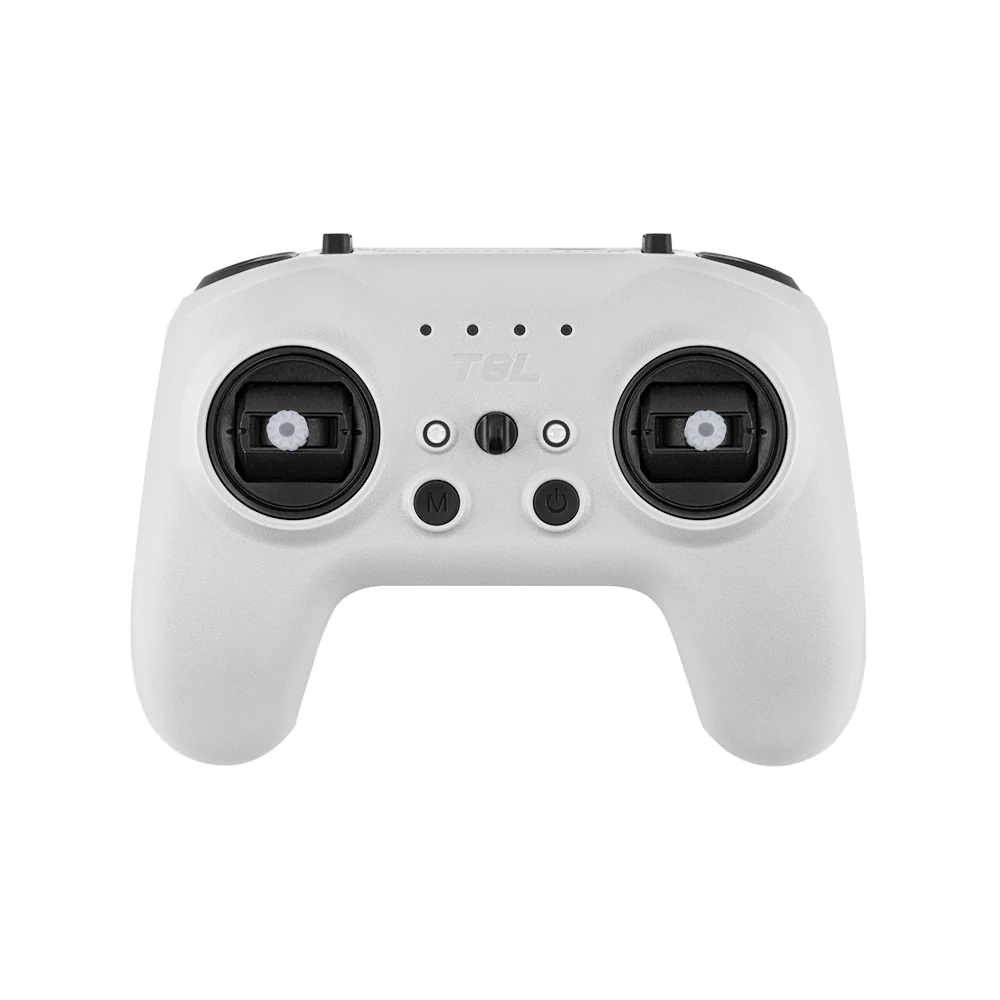
\includegraphics[width=\linewidth]{Bilder-Grafiken/Matthias/Fernsteuerung/T8L-RC-Controller.png}
    \captionof{figure}{Radiomaster T8L (M2) \cite{t8l_controller}}
\end{minipage}
\hfill
\begin{minipage}[c]{0.4\textwidth}
    \centering
    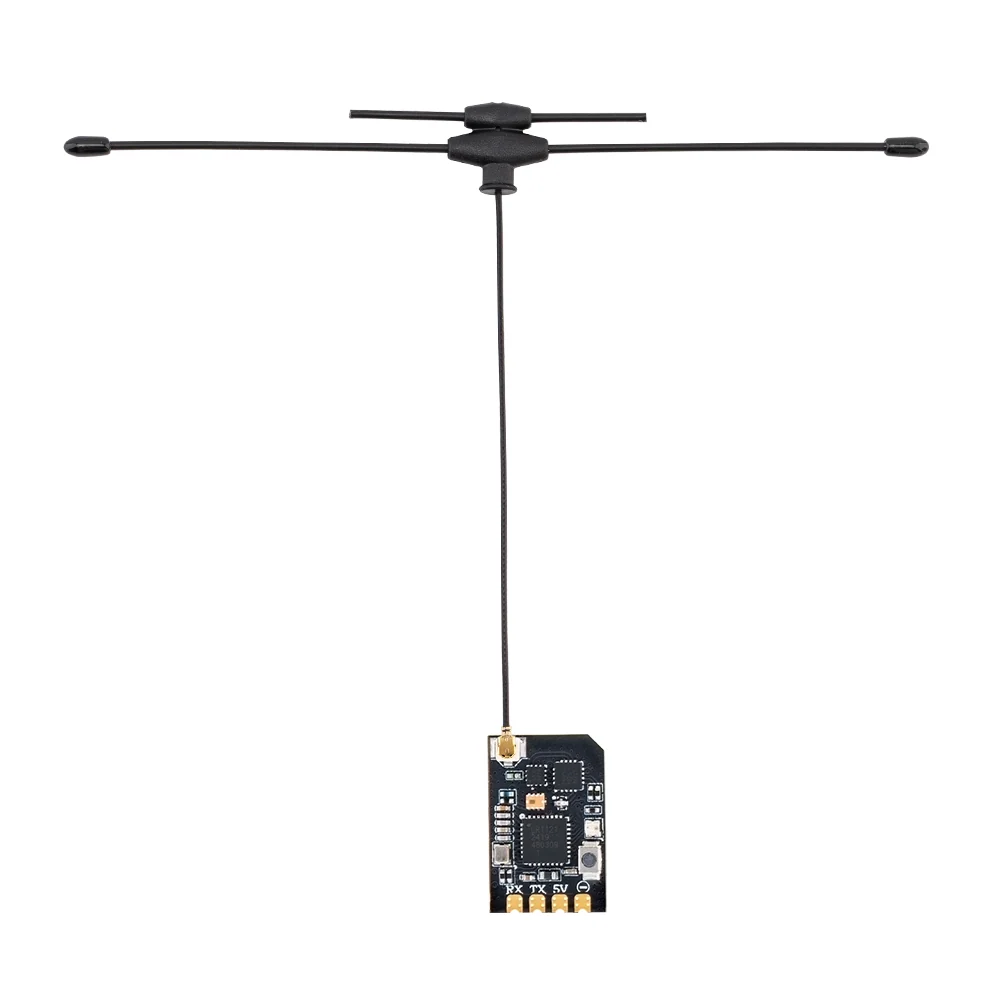
\includegraphics[width=\linewidth]{Bilder-Grafiken/Matthias/Fernsteuerung/XR1_Reciver_Bild.png}
    \captionof{figure}{Radiomaster XR1 Nano Multi-Frequency ExpressLRS Receiver
    \cite{XR1_reciver}}
\end{minipage}
\newpage
  


\section{CRSF-Protokoll}
CRSF ist ein Protokoll \cite{crsf_protokoll_spec} das für die Kommunikation von Radio Controlled (RC)
Geräten genutzt wird. Anders als wie bei z.B. S-Bus sind die Frame-Größen nicht
konstant, sondern werden auf Größe des Pakets angepasst. Das machte es zu einem
sehr flexiblen Protokoll, dass unter anderem die RC-Kanäle der Fernsteuerung, GPS
Daten und Übertragungsqualität übertragen kann, wie auch vieles weiteres.

\subsection{Aufbau eines Frames}
Der Anfang eines Frames ist immer gleich Aufgebaut. Es gibt einen Start Byte
(0xC8), Frame Länge und der Frame-Type. Danach folgt die Payload, die unterschiedlich lang
sein kann. Am Ende des Frames sitzt immer der CRC. Frames müssen mindestens 4
Byte lang sein und maximal 64 Byte.
\begin{figure}[h]
    \centering
    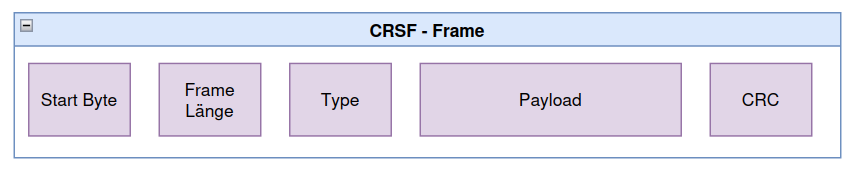
\includegraphics[width=\textwidth]{Bilder-Grafiken/Matthias/Fernsteuerung/CRSF-Frame.png}
    \caption{Aufbau des CRSF-Frames \cite{crsf_protokoll_spec}}
\end{figure}

\subsection{Protokoll Schnittstelle}
Das CRSF-Protokoll wird wie die meisten anderne RC-Fernsteuerungsprtokolle über
UART übertragen. In der CRSF-Specification \cite{crsf_protokoll_spec} werden
drei Arten der Schnittstellen beschrieben. \grqq Single-Wire Half-Duplex
UART\grqq, \grqq Dual-Wire Full-Duplex UART\grqq und \grqq Multi-master I2C
(BST)\grqq. Die Schnittstelle die der Radiomasterr XR1 Nano supported ist die
Full-Duplex UART schnittstelle.\\
Laut Specification ist diese defaultmäßig auf eine 416666 Baudrate, 8N1 (8 Daten
Bits, keine Parität, und in Stopp-Bit) eingestellt. Sie muss mit 3.0 - 3.3 Volt
betrieben werden. Das UART Signal ist nicht invertiert, anders wie bei anderen
RC-Protokollen (z.B. S-Bus).


\section{Architektur der CRSF-Protokollverarbeitung} 
Es wurde sich die Architektur und Implementation der CRSF-Protokollverarbeitung
bei Betaflight und Ardupilot analysiert. Betaflight ist \grqq die Weltweit
führende Multi-Rotor Flight-Controller Software\grqq.
Ardupilot ist ein Autopilot System das unterschiedliche arten
von Fahrzeugen supported. Beide sind Open Source. Es wurde sich damit befasst
wie diese zwei Projekte die Kommunikation mit dem RC-Receiver implementieren.

\newpage
\subsection{Betaflight}
Das Empfangen vom CRSF-Protokoll ist bei Betaflight Interrupt basiert
\cite{betaflight_crsf}.
Bei einem neu Empfangen Byte, löste der Rx-Interrupt aus. In diesem wird der
Byte in ein Statisches Array kopiert. Auch das Parsen wird direkt im 
Interrupt durchgeführt. In Abbildung
\ref{fig:flussdiagramm_betaflight} wird ein vereinfachter Ablauf 
der Interrupt Routine gezeigt. Wenn ein ganzes Frame Empfangen ist, wird
dieser im Scheduler weiter verarbeitet.

\begin{figure}[h]
    \centering
    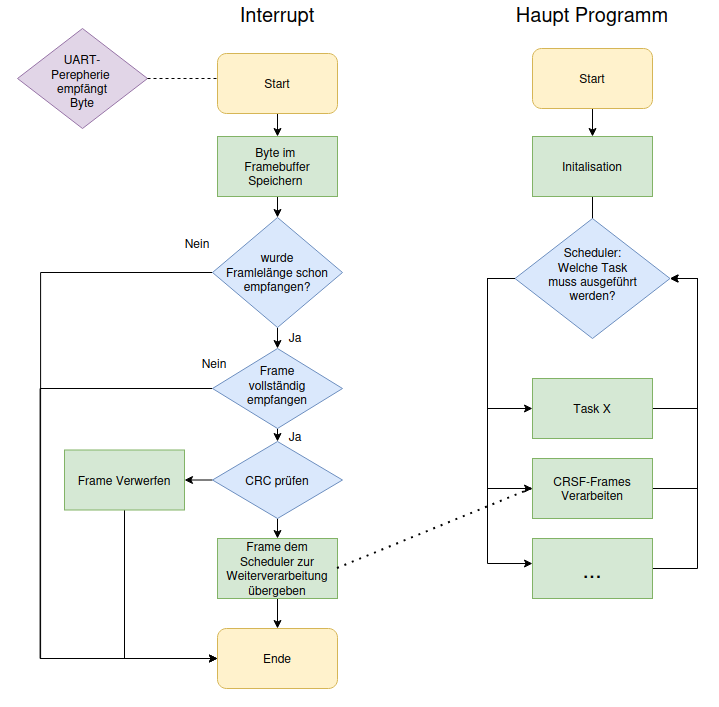
\includegraphics[width=0.95\textwidth]{Bilder-Grafiken/Matthias/Fernsteuerung/CRSF-Betaflight-Software.png}
    \caption{Betaflight - Empfang und Verarbeitung von CRSF-Frames}
    \label{fig:flussdiagramm_betaflight}
\end{figure}

\noindent
Erwähnenswert ist bei Betaflighs sehr viel des Empfangensprozess im Interrupt
verarbeitet. Die ISR im Sourcecode ist fast 150 Zeilen lang. Natürlich ist die
Zeilenanzahl ungleich der Ausführungszeit, veranschaulicht aber das sehr viel in
diesem Interrupt passiert. Das ist insoweit problematisch, da während des
Interrupts, der Prozessor auf nichts weiteres reagieren kann.

% --- BEGINN Ardupilot-Teil (von Claude eingefügt) ---
\newpage
\subsection{Ardupilot}
Anders als bei Betaflight nutzt Ardupilot eine DMA-Einheit
um den CRSF-Frame zu empfangen \cite{ardupilot_crsf}. Erst wenn ein
vollständiger Frame empfangen ist, wird ein sogenannter IDEL-Line-Interrupt
ausgelöst, mit diesem Interrupt wird die Verarbeitung gestartet.
Es ist zu erwähnen das Ardupilot ein Real time Operation System (RTOS) namens
ChibiOS nutzt. Die Verarbeitung der empfangenen Daten passiert in einer
Thread. In Abbildung
\ref{fig:flussdiagramm_ardupilot} wird ein vereinfachter Ablauf 
des Programmcodes gezeigt.

\begin{figure}[h]
    \centering
    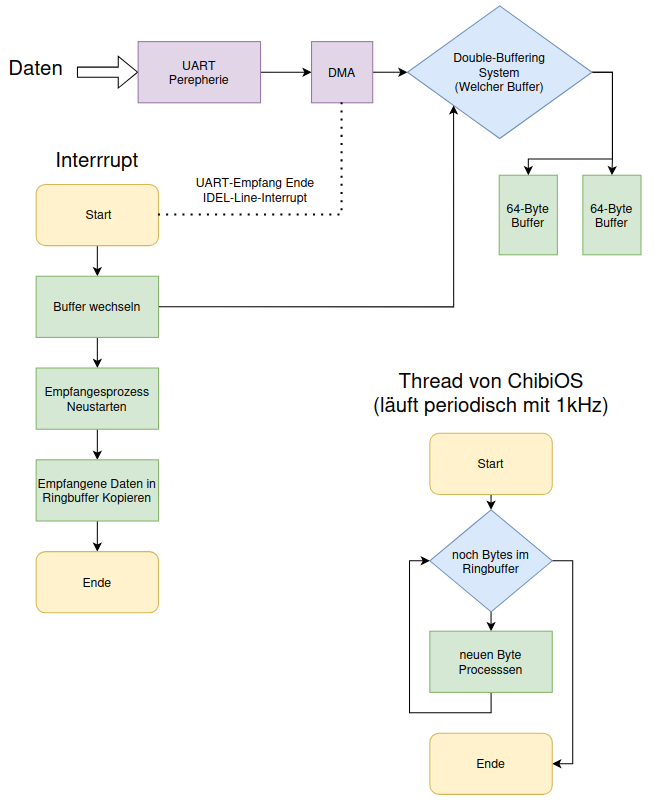
\includegraphics[width=0.75\textwidth]{Bilder-Grafiken/Matthias/Fernsteuerung/CRSF-Ardupilot-Software.png}
    \caption{Ardupilot - Empfang und Verarbeitung von CRSF-Frames}
    \label{fig:flussdiagramm_ardupilot}
\end{figure}

Da für den Empfang eine DMA-Einheit genugzt wird, wird die CPU gebraucht,
außer am Frame-Ende. Der ausgelöste Interrupt, wechselt den Buffer, in den
die DMA-Einheit schreibt, startet die Empfangensprozess neu und schreibt die
empfangenden Daten in einen seperaten Ringbuffer. Dieser Ringbuffer wird über
eine Thread in einem 1kHz Takt ausgelesen. Dadurch werden keine
Interrupts durch das Verarbeiten blockiert.

\subsection{Vergleich der Ansätze von Betaflight und Ardupilot}
Betaflight und Ardupilot nutzen verschiedene Ansätze zur Empfangung des
Protkolls. Betaflight verfolgt einen simplere Architektur, in der
alles über Interrupts verarbeitet wird. Erst wenn bestätigt ist, dass
sein Frame richtig empfangen wurde, wird die in dann durch eine Task in
einem Scheduler fertig verarbeitet. Ardupilot offloaded das Empfangen an rein
an die Hardware und nur einen kurzen Interrupt um den Empfangensprozess neu
zu starten. Das Verarbeiten wird rein in einer Thread
durchgeführt.\\
Ardupilot erzeugt somit weniger und dann kürzere Interrupts,
(zeit-)kritischere Interrupts blockieren könnte. Wobei es mit mehr Komplexität in der Implementierung folgt. 

\section{Gewählte Architektur für SmartDrive X4}
Bei der Implementierung wurde sich stark an Ardupilot orientiert. Es gibt aber
statt dem Doulbe-Buffering-System + Ringbuffer einen einzigen 512Byte großen 
Ring-Buffer, der direkt von der DMA-Einheit beschieben wird. Es werden nur bei Fehlern Interrupts
ausgelöst, der Rest wird im Hauptprogramm mit 100Hz verarbeitet. Pro Periode
werden alle neuen Daten geparsed, somit wird der aktuellste Frame jedes
Frametypen gespeichert. Dadurch das
alle Empfangen Daten im Buffer landen, ist das verarbeiten nicht Zeitkritisch.\\

Der Frame-Parser iteriert beim Start durch den Rinbbuffer bis er die Adresse für
Flight Contorller gefunden wird. Diese ist der Start des Frames. Alle Frame-Bytes
werden in einem Zwischen-Buffer gespeichert. Sobald das Ende des Frames erreicht
wurde, muss die Korrekte Übertragung mit der CRC-Checksumme überprüft werden.
Erst danach Kann der Frame-Inhalt verarbeitet werden. Dies muss für jeden
Fragetyp individuell getan werden. 

\begin{figure}[H]
    \centering
    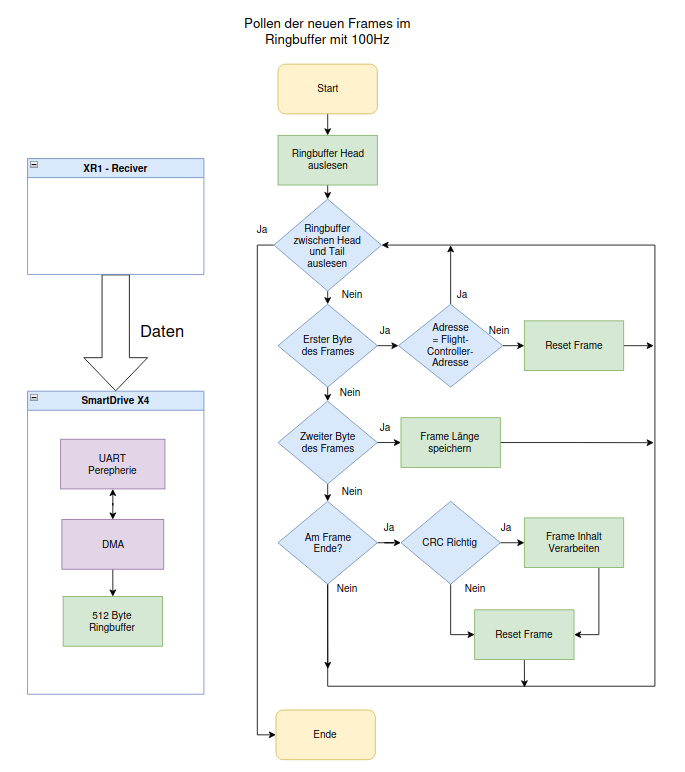
\includegraphics[width=1\textwidth]{Bilder-Grafiken/Matthias/Fernsteuerung/CRSF-SmartDriveX4-Software.png}
    \caption{Eigenimplementierung - Empfang und Verarbeitung von CRSF-Frames}
    \label{fig:flussdiagramm_smartdrivex4}
\end{figure}

\newpage

\subsubsection{Ring Buffer Dimensionierung}
Ein Problem dieses Buffers ist, dasss der Ringbuffer überlaufen kann.
Besonders wenn der Prozessor gerade andere rechenintensiven Teile des Programms
verarbeitet und dort aufgehalten wird. Daher muss der Buffer groß genug
gewählt werden, so dass genug reserve existiert um Verzögerungen in
der Verarbeitung ausgleichen zu können. Ein zu großer Buffer verschwendet
jedoch RAM.\\ 
Die Radiomaster T8L (M2) \cite{t8l_controller} und das CRSF-Protokoll unterstützt mehrere Update
Raten von 100Hz bis zu 1kHz. Diese sind am T8L einstellbar. Es muss der buffer für die Maximale Update
Frequenz und Frame-Größe dimensioniert werden. Es wurde folgende Formel
genutzt um die Zeit zu bestimmen, bis der Buffer überfüllt ist. Wobei:\\
$N_{Buf}$ ... Ringbuffer-Größe in Bytes\\
$n_{max}$ ... Maximale Frame-Größe in Bytes\\
$f$ ... Updaterate in Hz

\[
    T_{overflow} =\frac{N_{Buf}}{n_{max}} \cdot \frac{1}{f}
\] 

\[
    \frac{512 \text{Bytes}}{64 \text{Bytes}} \cdot \frac{1}{100 \text{Hz}} = 80ms
\] 
\[
    \frac{512 \text{Bytes}}{64 \text{Bytes}} \cdot \frac{1}{250 \text{Hz}} = 32ms
\] 
\[
    \frac{512 \text{Bytes}}{64 \text{Bytes}} \cdot \frac{1}{500 \text{Hz}} = 16ms
\] 
\[
    \frac{512 \text{Bytes}}{64 \text{Bytes}} \cdot \frac{1}{1 \text{kHz}} = 8ms
\] 
Aus diesen Rechnungen geht hervor, dass die Buffer-Größe bei 100Hz und 250Hz
ausreichend ist, wenn alle 10ms gepolled wird. Noch dazu muss eine gewisse Verzögerung
eingeplant werden, sie wurde mit unter 10ms angenommen. 
Ab 500Hz ist die $\text{Pollingzeit} + \text{Verzögerung}$ sehr knapp vor einem
Überlauf. Ab 1kHz ist die Buffer-Größe zu klein.\\
Es wurde trotzdem 512Bytes als Buffer-Größe gewählt, da in Theorie das
CRSF-Protokoll Übertragungsgeschwindigkeiten bis zu 1kHz supported. Dies kann am
Contorller eingestellt werden. Mehr als 250Hz wird in Praxis nicht gebraucht.\\
Die gewählte Formel beschreibt nur die Maximalauslastung. In Betrieb sind
die meisten Frames unter 64Bytes lang. Somit ist die Auslastung des Ringbuffers
geringer als berechnet.


\chapter{Inertial Measurement Unit (IMU)}
\chapterauthor{Matthias Greil}

\section{Grundlagenn der orientierungs Bestimmung} \label{Orientierung}

Die Orientierung eines Systems kann mit einer sogenannten Inertial Measurement Unit (IMU) gemessen werden. So eine IMU besteht tüpischerweise aus zwei/drei Sensoren: Gyroskop, Accelerometer und Magnetometer (optional). Jeder dieser Sensoren hat in der Anwendung Stärken wie auch Schwächen, deswegen werden sie Kombieniert umd die Orientierung mit wenig bis keinem Fehler bestimmen zu können. \\
Man spricht dabei über Sensor Fusion. Es handelt sich nicht um eine Mehtode sondern einen Überbegiff für verschiedene Algorithmen, wobei manche Simpler und weniger Leistungsintensiv im vergleich zu den anderen sind (Complimentär Filter) sind. Andere wie Madgwick, Mahony oder ein Kalman Filter, die implementierung und umsetzun komplizierter, aber dafür meist bessere ergebnise erziehlen können.

\subsubsection{Euler Winkel}
Euler Winkel sind eine Art eine Orientation in drei Dimensionalen Raum darzustellen\cite{EulerAngles}. Dabei wird die Rotation mit drei Achsen dargestellt. Diese Achsen werden in Schritten auf ein Modell angewendet. Rotation wird mit Winkeln $( \phi \, \theta \, \psi)$ dargestellt. Oft wird statt den Winkeln auch die namen Roll ($\psi$),Pich ($\theta$) und Yaw ($\phi$) benutzt. 
\begin{figure}[h]
    \centering
    \includegraphics[width=\textwidth]{Datasheet-Quellen/Bilder/eulerAngleBild.png}
    \caption{Anwendung von Euler Winkel Visualisiert \cite{eulerAnglesBild}}
\end{figure}

\subsection{Physiche Limitierungen von Sensoren}
In einem Idealen Szenario, gäbe es einen Sensor, der uns direkt seine Orientierung in allen drei Axen messen und ausgeben würde. Dies auch in einem Hochfrequenten Updaterate. In realität gibt es so einen Sensor nicht. Deswegen konbiniert man die Stärken von verschiedenen Sensorarten um die Ausrichtung eines Systems zu abzuschätzen.

\subsubsection{Gyroskop}
Ein sogenanntes Gyroscop misst die Winkelgeschwindigkeit (Veränderung der Orientierung) in allen drei Axen. Darus ist es möglich eine Relative Orientierung zu bestimmen, indem man die Messwerte integriet. Problem dabei ist, das der reale Sensor-Output einen Bias/Offset hat und ein Rauschen mitgemessen wird.\\
\textbf{Bias/Offset} ist ein konstanter Werte der bei jeder Messung mitgemessen wird. Der Bias variert vom einem Bauteil zum Nächsten, wie auch zwischen den Achsen. Jedoch ist es auch abhängig von der Temperatur des Sensors. Der Bias in den Messwerten ist beim Integriern ein Statischer Error und führt dazu das die berechnete Relative Orientation von der Wahren abdriftet.
Im Stillstand kann der Bias durch Mitteln von Messwerten bestimmt werden. Dieser Bias muss dann von jedem Messwert subtrahiert werden. 

\subsubsection{Accelerometer}
Ein sogenanntes Accelerometer misst die Beschleunigung eines Systems. In diesem Fall wird es hauptsächlich dafür genutzt die Erdgravitation zu messen, oder genauer gesagt einen Gravitationsvektor. Dieser Vektor wird dafür um ein absolutes Roll und Pitch des Sensros zu bestimmen. 

\subsubsection{Magnetometer} \label{magneto}
Ein Magnetometer oder auch manchmal eCompass genannt, misst die Stärk des Magnetfelder in den X-,Y- und Z-Achesn. Es wird dafür benutzt ein absoultes Yaw-Wert über das Erdmagnetfeldes errechnen zu können. Nachteile dafür sind, das Magnetometer typischerweise eine geringere Updaterate im vergleich zu Gyroskop und Accelerometer haben (typ nutzung 20 - 50Hz). Ein anderer Nachteil ist, dass ein Magnetometer nicht nur das Erdmagnetfeld misst, die Messwerte werden auch von allen ferromagnetischen Metallen, wie auch Magnetfeldern beeinflusst. Das Paper \textit{\grqq Calibration of Strapdown Magnetometers in the
Magnetic Field Domain\grqq} \cite[Sec.~2]{magCalThearie} beschreibt unteranderem die folgenden Einflüsse auf die Messwerte:
\begin{itemize}
    \item \textbf{Hardiron-Offset} beschreibt die Konstante Verzerrung des gemessenen. Dieser wird von feromagnetischen Metallen auf dem Fahrzeug verursacht.
    \item \textbf{Softiron-Offset} wird durch sogenannte \grqq soft iron\grqq Materialien verursacht. Diese Materialen verzerren die externen/zu messenden Magnetfelder (Erdmagnetfled) in Abhängigkeit zu sich selbst. Sind daher Orientierungsabhängig und nicht Konstant.
\end{itemize}
Diese Fehler können aus den Messwerten calibriert werden. Sind aber Umgebungsabhängig. Für die Anwendung in einem Fahrzeug bedeutet es, dass jedes mal neu calibiert werden muss, sobald sich der Aubau des Fahrzeuges verändert (Position des Magnetometer oder Struktureller Aubau des Fahrzeuges).

\subsection{Sensor Fusion}
Der Begriff Sensor Fusion beschreibt die Kombination von verschiedenen Arten von Sensoren. Dabei macht man sich die verschiedenen Stärken zu nutzen. Dabei wird das Gyroskop für das Erfassen von schnellen Änderungen genutzt. Das Accelerometer und Magnetometer hingegen werden typischerweise Tiefpassgefiltered und als absolute Refernez genutzt. Dabei gibt es nicht nur eine Art die Sensordaten zu kombinieren. Wie schon am Anfang von Kapitel \ref{Orientierung}. Dabei unterscheidet man zwischen 6 Achsen und 9 Achsen Fusion, dies beschreibt nur wie viele seperate Sensoren bei der Fusion benutzt wurden.
\begin{itemize}
    \item \textbf{6 Achsen Fusion}: Dabei werden nur Gyroskop und Accelerometer benutzt. Also 2 mal 3 Achsen. Dabei macht man sich wie schon zu vor erwähnt die Eigenschaften des Gyroskops zu nutzen für schnelle Bewegungen. Das Accelerometer wird dafür genutzt den Gravitationsvektor zu messen und so ein absoluten Roll- und Pitch-Wert zu haben. Wobei Yaw allein von dem Integrierten Gyroskopwert abhängt. Was ein Nachteil ist, wenn man eine konstante Heading benötigt.
    \item Bei der \textbf{9 Achsen Fusion} wird neben Gyroskop und Accelerometer auch das Magnetometer genutzt um ein konstantes Yaw-Wert errechnen zu können. Wie schon in Kapitel \ref{magneto} beschrieben muss dafür das Magnetometer kalibriert werden. Viele Systeme Fallen auf 6 Achsen Fusion zurück, falls das Magnetometer keine nützlichen Werte liefert. 
\end{itemize}

\subsubsection{Verwendete Sensor Fusion Algorithmus}
Um die Komplexität des verwendeten Fiters gering zu halten, wurde die MotionFX Libary von St Microelectronics \cite{st_motionFX} genugzt. Diese Laut der Dokumentation einen Kalman Filter intern, aber ist für den nutzer eine Black Box. Da wir schon mit St's Entwicklungsumgebung arbeiten, war es die einfachste möglichkeit Sensor Fusion zu implementieren. Wie in Kapitel \ref{imuWahl} genauer erkärt, wurde für das Smart Drive X4 speziell auf eine gute 6 Achsen Fusion Wert gelegt. Diese wurde dann direkt mit dem SFLP-Core des LSM6DSV16X berechnet.Dies ist die Fallback Fusion falls das Magnetometer keine nützlichen Daten liefert. Im regelfall wurde die MotionFX dafür genutzt, im 9 Achsen Fusion Modus.\\
\newpage

\section{Wahl der IMU} \label{imuWahl}
Das primäre Ziel für die IMU war die Möglichkeit die Heading möglichst genau zu
bestimmen. Im Vordergrund stand dabei eine hochwertige 6-Achsen-Fusion aus
Gyroskop und Accelerometer. Es sollte aber auch die Möglichkeit einer
9-Achsen-Fusion bestehen. Da aber nicht nicht Sicherstellbar im Anwendungsfall
von Smart Drive X4 die Nutzung von einem Magnetometer möglich sein könnte,
wurde besonders auf eine Solide 6 Achsen Fusion wert gelegt. Grund hierfür ist,
dass im Fahrzeug durch den Einsatz von Motoren, Stromleitungen sowie
ferromagnetischen Komponenten, dass die Messwerte des Magnetometer liefern kann
(vgl. Hardiron- und Softiron-Effekte im vorangegangenen Kapitel).
Verwertbare Messwerte liefert (vgl. Hard- und Softiron-Effekte im
vorangegangenen Kapitel).\\

\begin{minipage}[c]{0.55\textwidth}
\subsection{Gewählte IMU: LSM6DSV16X}
Die Wahl fiel auf die \textit{LSM6DSV16X} von STMicroelectronics. Sie ist eine
6 Achsen IMU und zeichnet sich besonders über ihre Low-Noice-Charakteristik aus,
wie auch den internen Motion-Processor (SFLP-Block). Diese Sensor Fusion Low
Power Einheit (SFLP) liefert unter anderem einen Game Rotation Vektor in
Quaternion Format und Gyro-Bias-Calibration. Alle Sensordaten und Fusiondaten des SFLP-Blocks können in
den internen FIFO. Dabei wird alles in Batches zusammengefasst und kann mit
einem Zeitstempel versehen werden.\\
Weiters verfügt der \textit{LSM6DSV16X} über eine Sensor-Hub-Funktionalität. 
Dabei agiert die IMU als I2C-Master und kann externe Sensoren auslesen. 
Diese Funktion wurde dafür genutzt werden ein externes Magnetometer an zu schließen,
die Messwerte über im FIFO zu speichern und diesen aus zu lesen.
Dies ist hilfreich weil alle Sensordaten an einem Zentralen Punkt ausgelesen werden konnten.
\end{minipage}
\hfill
\begin{minipage}[c]{0.4\textwidth}
    \centering
    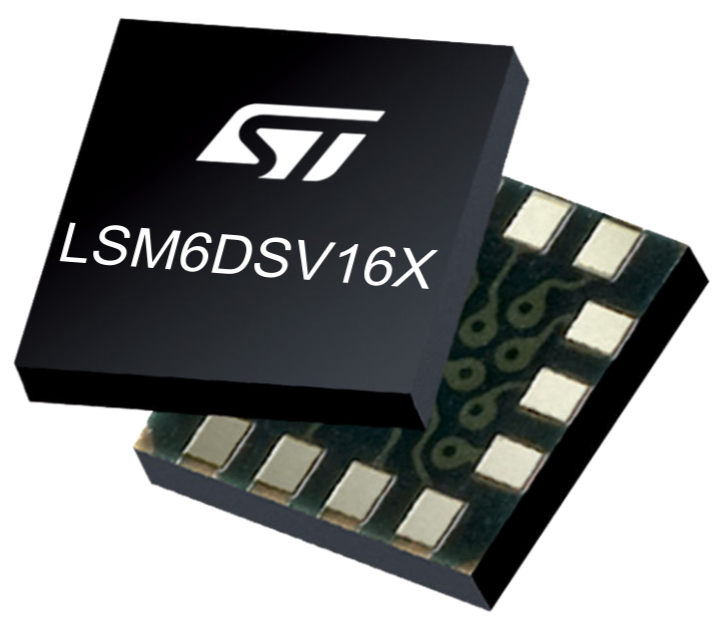
\includegraphics[width=\linewidth]{Bilder-Grafiken/Matthias/IMU/LSM6DSV16X_Package_Image.png}
    \captionof{figure}{LSM6DSV16X von STMicroelectronics, 6-Achsen IMU \cite{st_lsm6dsv16x}}
\end{minipage}

\subsection{Betrachtete Alternativen}
Als Alternativen wurden die \textit{ICM-42688-P} von TDK InvenSense \cite{tdk_icm42688p}
sowie die \textit{BNO086} von CEVA \cite{ceva_bno08x} evaluiert.
Die \textit{ICM-42688-P} ist eine 6 Achsen IMU mit ähnliche Low-Noice-Charakteristik
und Preis wie die \textit{LSM6DSV16X}, aber keinen internen Motion Processor und
Sensor-Hub. Die \textit{BNO086} ist eine 9 Achsen IMU mit integriertem 
32bit ARM Cortex-M0+ Core für Sensorfusion und Calibration.
Damit ist sie deutlich komplexer und auch
teurer. Noch dazu ist der interne Processor eine Black Box. \\
Es wurde die \textit{LSM6DSV16X} gewählt weil sie im Vergleich zu der
\textit{BNO086} mehr Flexibilität bietet, jedoch mehr features wie die
\textit{ICM-42688-P} bietet.

\section{Wahl des Magnetometers}
Für die angestrebte 9-Achsen-Fusion ist ein zusätzliches Magnetometer
erforderlich. Wie schon erwähnt, kann die \textit{LSM6DSV16X} als Sensor-Hub
agieren. STMicroelectronics selbst bietet ein Example an, bei das
\textit{LIS2MDL} Magnetometer über den Sensor-Hub ausgelesen wird. Für Smart
Drive X4 wurde die \textit{LIS2MDL} gewählt, da die Implementierung durch die
Beispiele schon existierte und dies somit keine Eigenimplementation erfolgen
muss. 





\printbibliography

\end{document}
